\documentclass[tikz, border=3mm]{standalone}

% Packages principaux
\usepackage{tikz}
\usepackage[european, straightvoltages, RPvoltages, cute inductors]{circuitikz}
\usepackage{smartdiagram}
\usepackage{couleurs-fr}
\usepackage{xcolor}
\usepackage{tcolorbox}

% Bibliothèques TikZ
\usetikzlibrary{
	shapes.geometric,
	arrows.meta,
	arrows,
	shadows.blur,
	positioning,
	decorations.pathreplacing,
	decorations.markings,
	calc
}

% Styles TikZ personnalisés
\tikzstyle{block} = [rectangle, rounded corners, minimum height=3em, minimum width=4em, text centered, draw=black, fill=green!30]
\tikzstyle{arrow} = [very thick, draw=green, -{Stealth[color=green, fill=black, width=8pt, length=10pt]}]
\tikzstyle{info} = [rectangle, minimum height=2em, minimum width=2cm, text centered]
\tikzstyle{process} = [rectangle, minimum width=2cm, minimum height=1.5cm, text centered, draw=black, text=black, align=center, aspect=2]

\begin{document}
	
	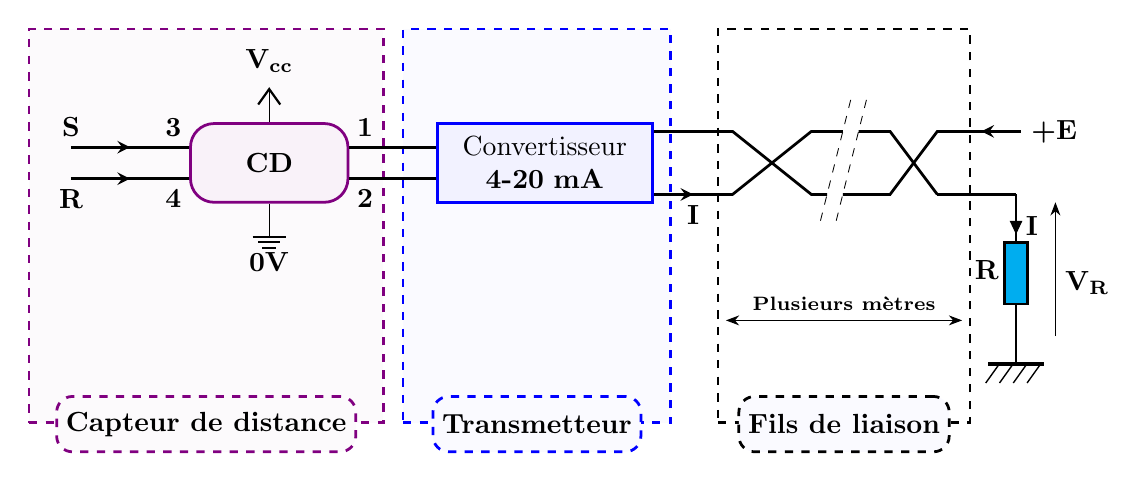
\begin{tikzpicture}
		
		% Réglages circuitikz
		\ctikzset{
			amplifiers/fill=cyan,
			sources/fill=green,
			diodes/fill=red,
			resistors/fill=violet,
			resistors/scale=0.7,
		}
		
		% ====== Bloc Capteur ======
		\node[draw=violet, minimum width=4.5cm, minimum height=5cm, anchor=center,
		dashed, rounded corners=0.0cm, line width=1pt,
		drop shadow={shadow xshift=0mm, shadow yshift=-0mm, opacity=0.1},
		fill=violet!2, text width=1cm, align=center] 
		(hg1) at (-0.8,5.2) {};
		
		\node[info, fill=violet!2, draw=violet, rounded corners=0.2cm, line width=1pt, dashed]
		at (hg1.south) {\textbf{Capteur de distance}};
		
		% ====== Bloc Transmetteur ======
		\node[draw=blue, minimum width=3.4cm, minimum height=5cm, anchor=center,
		dashed, rounded corners=0.0cm, line width=1pt,
		drop shadow={shadow xshift=0mm, shadow yshift=-0mm, opacity=0.1},
		fill=blue!2, text width=1cm, align=center] 
		(hg2) at (3.4,5.2) {};
		
		\node[info, fill=blue!2, draw=blue, rounded corners=0.2cm, line width=1pt, dashed]
		at (hg2.south) {\textbf{Transmetteur}};
		
		% ====== Bloc Fils de liaison ======
		\node[draw=black, minimum width=3.2cm, minimum height=5cm, anchor=center,
		dashed, rounded corners=0.0cm, line width=1pt,
		drop shadow={shadow xshift=0mm, shadow yshift=-0mm, opacity=0.1},
		fill=blue!0, text width=1cm, align=center] 
		(hg3) at (7.3,5.2) {};
		
		\node[info, fill=blue!2, draw=black, rounded corners=0.2cm, line width=1pt, dashed]
		at (hg3.south) {\textbf{Fils de liaison}};
		
		% ====== Distance entre blocs ======
		\draw[<->, >=Stealth, font={\scriptsize}, fill=white] 
		(5.8,4) -- (8.8,4) node[midway, above] {\textbf{Plusieurs mètres}};
		
		% ====== Capteur CD ======
		\node[draw=violet, minimum width=2cm, minimum height=1cm, anchor=center,
		rounded corners=0.3cm, line width=1pt,
		drop shadow={shadow xshift=0mm, shadow yshift=-0mm, opacity=0.1},
		fill=violet!5, text width=1cm, align=center]
		(cd) at (0,6) {\textbf{CD}};
		
		% Signaux S et R
		\draw[postaction=decorate, line width=1pt, decoration={markings, mark=at position 0.5 with {\arrow{stealth}}}]
		(cd.west)+(-1.5,0.2) node[above]{\textbf{S}} -- ++(0,0.2) node[above,xshift=-0.2cm]{\textbf{3}};
		
		\draw[postaction=decorate, line width=1pt, decoration={markings, mark=at position 0.5 with {\arrow{stealth}}}]
		(cd.west)+(-1.5,-0.2) node[below]{\textbf{R}} -- ++(0,-0.2) node[below,xshift=-0.2cm]{\textbf{4}};
		
		% Alimentation
		\node[vcc] (VCC) at (cd.north) {$\mathbf{V_{cc}}$};
		\draw (cd.south) node[ground] (Gnd) {} node[below=0.5cm] {$\mathbf{0V}$};
		
		% ====== Convertisseur 4-20mA ======
		\node[draw=blue, minimum width=2cm, minimum height=1cm, anchor=center,
		rounded corners=0.0cm, line width=1pt,
		drop shadow={shadow xshift=0mm, shadow yshift=-0mm, opacity=0.1},
		fill=blue!5, text width=2.5cm, align=center]
		(conv) at (3.5,6) {Convertisseur\\ \textbf{4-20 mA}};
		
		\draw[line width=1pt] (cd.east)+(0,-0.2) node[below,xshift=0.2cm]{\textbf{2}} -- ($(conv.west)+(0,-0.2)$);
		\draw[line width=1pt] (cd.east)+(0,0.2) node[above,xshift=0.2cm]{\textbf{1}} -- ($(conv.west)+(0,0.2)$);
		
		% ====== Câblage courant I ======
		\draw[postaction=decorate, line width=1pt, decoration={markings, mark=at position 0.5 with {\arrow{stealth}}}]
		(conv.east)+(0,-0.4) --++ (1,-0.4) node[below,xshift=-0.5cm]{\textbf{I}} coordinate(t);
		
		\draw[line width=1pt] (conv.east)+(0,0.4) --++(1,0.4)--++(1,-0.8)--++(0.2,0) coordinate(t1);
		\draw[line width=1pt] ($(t)-(0.1,0)$) -- (t) --++(1,0.8)--++(0.4,0) coordinate(t2);
		
		% Connexions vers résistance
		\draw[line width=1pt] ($(t2)+(0.2,0)$) coordinate(t3) --++(0.4,0)--++(0.6,-0.8) coordinate(g);
		\draw[line width=1pt] ($(t1)+(0.2,0)$) coordinate(t4) --++(0.6,0)--++(0.6,0.8)--++(0.06,0) coordinate(g1);
		
		\draw[dashed, line width=0.3pt] ($(t3)!-0.5!(t4)$) -- ($(t3)!1.5!(t4)$);
		\draw[dashed, line width=0.3pt] ($(t2)!-0.5!(t1)$) -- ($(t2)!1.5!(t1)$);
		
		\draw[postaction=decorate, line width=1pt, decoration={markings, mark=at position 0.5 with {\arrow{stealth}}}]
		($(g1)+(1,0)$) node[right]{\textbf{+E}} --++ (-1,0);
		
		\draw[line width=1pt, short, -*] (g) --++(1,0) coordinate(ff);
		\draw (ff) --++(0,-0.2) to[line width=0.5pt, R, fill=cyan, l_=$\mathbf{R}$, i>^=$\mathbf{I}$] ++(0,-1.6) node[eground] {};
		
		\draw[-Stealth] ($(g)-(-1.5,1.8)$) --++ (0,1.7) node[pos=0.4, right] {$\mathbf{V_R}$};
		
	\end{tikzpicture}
	
\end{document}
